\section{Distress Cover}

\begin{figure}[htbp]
\centering
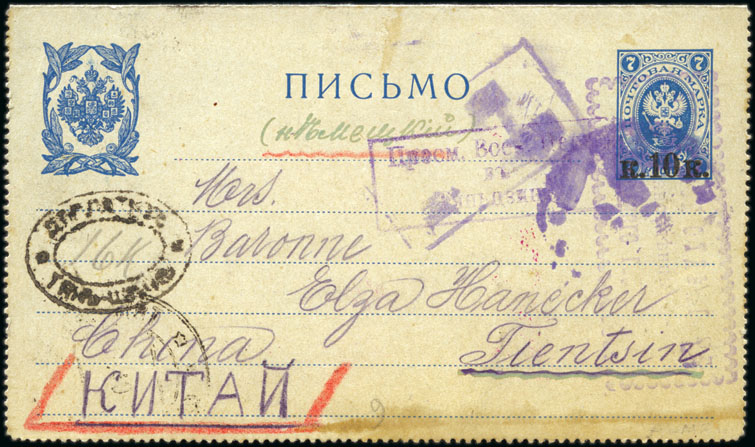
\includegraphics[width=.95\textwidth]{../russian-post-offices-in-china/10018.jpg}
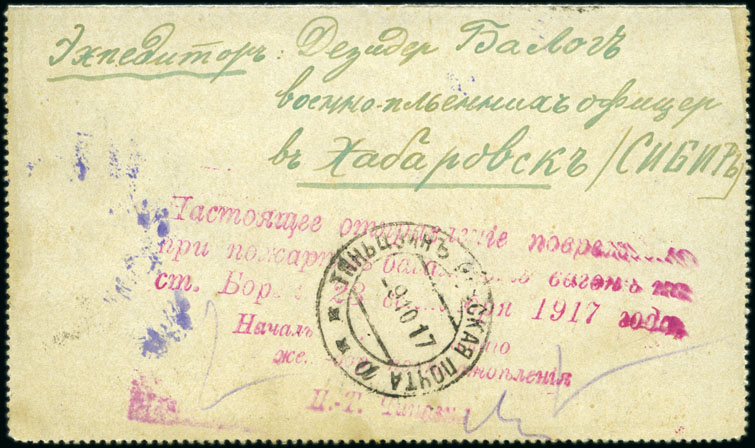
\includegraphics[width=.95\textwidth]{../russian-post-offices-in-china/10018-1.jpg}

\caption{
10018	TIENTSIN: 1917 10k on 7k provisional postcard sent by a German 
officer in the P.O.W. camp at Khabarovsk (Siberia) to Tientsin, cancelled by 
illegible cds and ornamental framed "Postal Division / Prisoners of War / 
Khabarovsk Garrison" cachet, both in violet, received at Tientsin 9.10.17 
(T\&S type 6 cds) and struck with two censor hs and oval "Dopltatit / 
Tientsin" (To Pay) hs with ms 16k, reverse with six-line
"Received by the Sending (Department) Damaged / By Fire in the Baggage (Car) 
on the Train at / Station Borzya 23 September 1917 / Manager/Railway Postal 
Department / Post Telegraph Clerk..." cachet, described in the
"British Journal of Russian Philately" no.31 (1962) as the first 
recorded Russian wreck cover, Tientsin "Doplatit" unrecorded by T\&S, 
unique showpiece.
\euro 2,000.00
}  
\end{figure}





                                                                      